% \documentclass[handout]{beamer}
\documentclass{beamer}

\mode<presentation>
{
  \usetheme{default}
  \usefonttheme[onlymath]{serif}
  % \usetheme{Singapore}
  % \usetheme{Warsaw}
  % \usetheme{Malmoe}
  % \useinnertheme{circles}
  % \useoutertheme{infolines}
  % \useinnertheme{rounded}

  \setbeamercovered{transparent=10}
}

\usepackage[english]{babel}
\usepackage[latin1]{inputenc}
\usepackage{alltt,listings,multirow,ulem,siunitx}
\usepackage[absolute,overlay]{textpos}
\TPGrid{1}{1}
\usepackage{pdfpages}
\usepackage{multimedia}
\usepackage{multicol}
\newcommand\hmmax{0}
\newcommand\bmmax{0}
\usepackage{bm}
\usepackage{comment}

% font definitions, try \usepackage{ae} instead of the following
% three lines if you don't like this look
\usepackage{mathptmx}
\usepackage[scaled=.90]{helvet}
% \usepackage{courier}
\usepackage[T1]{fontenc}
\usepackage{tikz}
\usetikzlibrary{decorations.pathreplacing}
\usetikzlibrary{shadows,arrows,shapes.misc,shapes.arrows,shapes.multipart,arrows,decorations.pathmorphing,backgrounds,positioning,fit,petri,calc,shadows,chains,matrix}


% \usepackage{pgfpages}
% \pgfpagesuselayout{4 on 1}[a4paper,landscape,border shrink=5mm]

\usepackage{JedMacros}

\newcommand{\timeR}{t_{\mathrm{R}}}
\newcommand{\timeW}{t_{\mathrm{W}}}
\newcommand{\mglevel}{\ensuremath{\ell}}
\newcommand{\mglevelcp}{\ensuremath{\mglevel_{\mathrm{cp}}}}
\newcommand{\mglevelcoarse}{\ensuremath{\mglevel_{\mathrm{coarse}}}}
\newcommand{\mglevelfine}{\ensuremath{\mglevel_{\mathrm{fine}}}}

%solution and residual
\newcommand{\vx}{\ensuremath{x}}
\newcommand{\vc}{\ensuremath{\hat{x}}}
\newcommand{\vr}{\ensuremath{r}}
\newcommand{\vb}{\ensuremath{b}}

\renewcommand{\vs}{\mathbf{s}}
\newcommand{\vz}{\mathbf{z}}
% \newcommand{\vy}{\mathbf{y}}
\newcommand{\vu}{\mathbf{u}}
\newcommand{\vw}{\mathbf{w}}
% %\newcommand{\vf}{\mathbf{f}}
\newcommand{\vF}{\mathbf{F}}
\newcommand{\vG}{\mathbf{G}}
\newcommand{\vJ}{\mathbf{J}}
% \newcommand{\vM}{\mathbf{M}}
% \newcommand{\vY}{\mathbf{Y}}
\newcommand{\vI}{\mathbf{I}}
% \newcommand{\vE}{\mathbf{E}}

\title{Low-rank Quasi-Newton Updates for Robust Jacobian Lagging in Newton Methods}
\author{{\bf Jed Brown} and Peter Brune}

% - Use the \inst command only if there are several affiliations.
% - Keep it simple, no one is interested in your street address.
\institute
{
  {Mathematics and Computer Science Division, Argonne National Laboratory}
}

\date{ANS M\&C, 2013-05-08}

% This is only inserted into the PDF information catalog. Can be left
% out.
\subject{Talks}


% If you have a file called "university-logo-filename.xxx", where xxx
% is a graphic format that can be processed by latex or pdflatex,
% resp., then you can add a logo as follows:

% \pgfdeclareimage[height=0.5cm]{university-logo}{university-logo-filename}
% \logo{\pgfuseimage{university-logo}}



% Delete this, if you do not want the table of contents to pop up at
% the beginning of each subsection:
% \AtBeginSubsection[]
% {
% \begin{frame}<beamer>
%   \frametitle{Outline}
%   \tableofcontents[currentsection,currentsubsection]
% \end{frame}
% }

\AtBeginSection[]
{
  \begin{frame}<beamer>
    \frametitle{Outline}
    \tableofcontents[currentsection]
  \end{frame}
}

% If you wish to uncover everything in a step-wise fashion, uncomment
% the following command:

% \beamerdefaultoverlayspecification{<+->}

\begin{document}
\lstset{language=C}
\normalem

\begin{frame}
  \titlepage
\end{frame}

\begin{frame}{What makes a nonlinear algebraic problem difficult?}
  \begin{itemize}
  \item Ill-conditioning
    \begin{itemize}
    \item For a second order elliptic problem, condition number $\sim \bigO(h^{-2})$.
    \item Anisotropy, and coefficient structure make the issue worse
    \item Iterative algorithms with local corrections cannot fix these asymptotics
    \item Eventual convergence guaranteed for many methods (in exact arithmetic)
    \item Practical convergence too slow, worse in parallel
    \end{itemize}
  \item Nonlinearity (especially non-smoothness)
    \begin{itemize}
    \item Plasticity, contact, shocks, phase change, bifurcations
    \item Usually local (in some sense), but can have long-range effects
    \item Methods stop converging as parameters change
    \end{itemize}
  \item<2> Nonlinearity interacts with ill-conditioning
  \end{itemize}
\end{frame}

\begin{frame}{Why global linearization?}
  \begin{itemize}
  \item Reuse of algorithms and software
    \begin{itemize}
    \item Sparse matrices help decouple software
    \item Many preconditioners can operate directly on 
    \end{itemize}
  \item Debugging discretization and singular behavior
    \begin{itemize}
    \item Compare to finite difference Jacobian
    \item Direct solves, singular values
    \end{itemize}
  \item Convergence theory
  \item Amortize setup costs
    \begin{itemize}
    \item Evaluate material models once
    \item Solve linear problem without re-evaluating
    \end{itemize}
  \item Algorithms that are not available without linearization
    \begin{itemize}
    \item Direct solvers
    \item Coarsening for algebraic multigrid
    \end{itemize}
  \item For irregular problems, convergent nonlinear iterations 
  \end{itemize}
\end{frame}

\begin{frame}{Inexact Newton methods}
  \begin{textblock}{0.18}[1,0](0.99,0)
    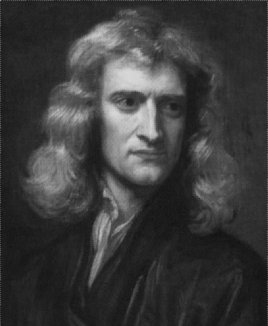
\includegraphics[width=\textwidth]{figures/Newton}
  \end{textblock}
  \begin{itemize}
  \item Standard form of a nonlinear system
    \[ \vF(\vu) = 0 \]
  \item Iteration
    \begin{align*}
      \text{Solve:} & \qquad \vJ(\vu) \vw = -\vF(\vu) \qquad (\text{Krylov}) \\
      \text{Update:} & \qquad \vu^+ \gets \vu + \lambda \vw
    \end{align*}
    \item Quadratically convergent near root: $\abs{\vu^{n+1}-\vu^*} \in \bigO\Big(\abs{\vu^n-\vu^*}^2\Big)$
    \item Picard is the same operation with a different $\vJ(\vu)$
  \end{itemize}
  % \begin{example}[Nonlinear Poisson]
  %   \begin{align*}
  %     \vF(\vu)=0 \quad &\sim\quad -\div\big[ (1+\vu^2) \grad \vu \big] - f = 0 \\
  %     \vJ(\vu)\vw \quad &\sim\quad  -\div\big[(1+\vu^2)\grad \vw + 2uw\grad \vu \Big]
  %   \end{align*}
  % \end{example}
  \begin{example}[$\mathfrak p$-Bratu]
    Suppose $\vF(\vu)$ is a discretization of \vspace{-1em}
    \[ -\nabla \cdot \big( \eta \nabla u \big) - \lambda e^u - f = 0, \qquad \eta(\gamma) = (\epsilon^2+\gamma)^{\frac{\pfrak-2}{2}}, \quad \gamma = \half \abs{\nabla u}^2 . \]
    Then $\vJ(\vu)\vw$ is a discretization of  \vspace{-1em}
    \[ -\nabla \cdot \big[ (\eta \bm 1 + \eta' \nabla u \otimes \nabla u) \nabla w \big] - \lambda e^{u} w . \]
  \end{example}
\end{frame}

\begin{frame}{Bottlenecks of (Jacobian-free) Newton-Krylov}
  \begin{columns}
    \begin{column}{0.4\textwidth}
      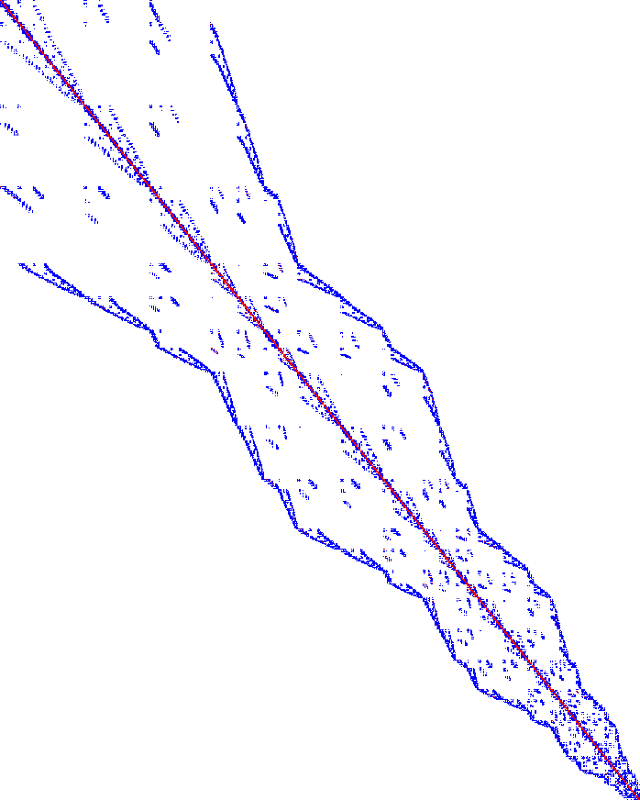
\includegraphics[width=1.15\textwidth]{figures/Dohp/EllipRCM}
    \end{column}
    \begin{column}{0.6\textwidth}
      \begin{itemize}
      \item Matrix assembly
        \begin{itemize}
        \item integration/fluxes: FPU
        \item insertion: memory/branching
        \end{itemize}
      \item Preconditioner setup
        \begin{itemize}
        \item coarse level operators
        \item overlapping subdomains
        \item (incomplete) factorization
        \end{itemize}
      \item Preconditioner application
        \begin{itemize}
        \item triangular solves/relaxation: memory
        \item coarse levels: network latency
        \end{itemize}
      \item Matrix multiplication
        \begin{itemize}
        \item Sparse storage: memory
        \item Matrix-free: FPU
        \end{itemize}
      \item Globalization
      \end{itemize}
    \end{column}
  \end{columns}
\end{frame}


\begin{frame}{Lagging}
  \begin{itemize}
  \item Lag the Jacobian (Shamanskii)
    \begin{itemize}
    \item Solve $\vJ(\vu_{\text{old}}) \vw = - \vF(\vu)$
    \item[X] Less robust: $\vw$ may not be a descent direction
    \item[X] Gives up quadratic convergence, but if $\vu_{\text{old}}$ is updated every $m$ steps, terminal convergence is superlinear
    \end{itemize}
  \item JFNK with lagged preconditioner
    \begin{itemize}
    \item Approximate $\vJ_{\text{mf}}(\vu)\vw = \frac{\vF(\vu+\epsilon \vw) - \vF(\vu)}{\epsilon}$ for chosen $\epsilon$
    \item Occasionally to build preconditioner $P_{\text{old}} = \mathcal{P}\big[\vJ(\vu_{\text{old}})\big]$ using assembled operator
    \item Iteratively solve: $P_{\text{old}}^{-1} \vJ_{\text{mf}}(\vu) \vw = - P_{\text{old}}^{-1} \vF(\vu)$
    \item Same robust nonlinear convergence of standard Newton
    \item[X] Residual $\vF$ is evaluated in every Krylov iteration
    \item[X] Number of Krylov iterations increases when $P_{\text{old}}$ becomes stale
    \item[X] Finite differencing noisy for ill-conditioned problems, sensitive to $\epsilon$
    \end{itemize}
  \end{itemize}
\end{frame}

\begin{frame}{Line Search: a scalar example}
  Minimize: $f(x) = x^2 - \exp(-4 (x-2)^2)$, gradient $\vF(x) = \partial f/\partial x$
  \includegraphics<1>[width=0.5\textwidth]{figures/LineSearch/SimpleExample}
  \includegraphics<2>[width=0.5\textwidth]{figures/LineSearch/SimpleReformulatedOptimization}
  \uncover{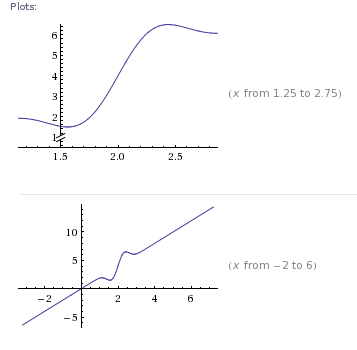
\includegraphics[width=0.5\textwidth]{figures/LineSearch/SimpleGradient}}
  \begin{itemize} \vspace{-1ex}
  \item Minimization problem with a unique minimum
  \item What if we can't evaluate ``objective'' functional? \\
    Root-finding problem with unique solution, but with singular points
  \item<2> $\hat f(x) = \norm{\vF(x)}^2$ \alert{Minimization problem with multiple minima}
  \end{itemize}
\end{frame}

\begin{frame}{Line Search}
  \begin{itemize}
  \item Backtracking: search in the 2-norm of the residual
    \begin{itemize}
    \item Find $\lambda$ such that $\norm{\vF(\vu + \lambda \vw)} < \norm{\vF(\vu)}$
    \item Shorten using polynomial fit of recently-evaluated $\lambda$
    \item Richardson (gradient descent) fails for a non-convex minimization problem
    \item Requires no extra function evaluations if $\lambda=1$ provides sufficient decrease
    \end{itemize}
  \item Critical point line search: locally consistent with minimization problem
    \begin{itemize}
    \item Start with descent direction: $\vw^T \vF(\vu) < 0$
    \item Find $\lambda$ such that $\vw^T \vF(\vu + \lambda \vw) = 0$ (use secant method in $\lambda$)
    \item Satisfies the second Wolfe condition
    \item Requires two residual evaluations in best case
    \end{itemize}
  \end{itemize}
\end{frame}

\begin{frame}{Quasi-Newton: Low-rank updates to $\vJ(\vu_{\text{old}})^{-1}$}
  \begin{equation*}
    \tilde \vJ_i(\vu_{\text{old}}) \vw = - \vF(\vu)
  \end{equation*}
  \begin{itemize}
  \item $\vs_i = \vu_i - \vu_{i-1}$, \quad $z_i = \vF(\vu_i) - \vF(\vu_{i-1})$, \quad $\vJ_0^{-1} = \mathcal{P}\big[\vJ(\vu_{\text{old}})\big]^{-1}$
  \end{itemize}
  \begin{description}
  \item[Broyden] Rank-1 update to the inverse Jacobian
    \begin{equation*}
      \tilde{\vJ}_{i}^{-1} = (\vI + \frac{(\vs_{i}-\tilde{\vJ}^{-1}_{i-1}\vz_{i}\vs_{i}^{\top})}{\vs_{i}^\top \tilde{\vJ}^{-1}_{i-1}\vz_{i}})
                     \tilde{\vJ}^{-1}_{i-1}.\
    \end{equation*}
  \item[BFGS] Broyden-Fletcher-Goldfarb-Shanno, a symmetric rank-2 update
    \begin{equation*}
      \tilde{\vJ}_{i}^{-1} = (\vI - \frac{\vs_{i} \vz_{i}^{\top}}{\vs_{i}^\top \vz_{i}})
                     \tilde{\vJ}^{-1}_{i-1}
                     (\vI - \frac{\vz_{i} \vs_{i}^{\top}}{\vs_{i}^{\top} \vz_{i}}) + \frac{\vs_{i}\vs_{i}^{\top}}{\vs_{i}^{\top}\vz_{i}},
    \end{equation*}
    \begin{itemize}
    \item For linear problems: equivalent convergence rate to conjugate gradients
    \end{itemize}
  \end{description}
\end{frame}

\begin{frame}{Quasi-Newton was born in the optimization world}
  \begin{itemize}
  \item Broyden's method is nearly 50 years old.
  \item Hessian information is often not available in optimization
    \begin{itemize}
    \item $J_0$ is very simple (diagonal, often the identity)
    \item Quasi-Newton is used to build a better approximation
    \item Restart occasionally to limit memory usage
    \item More like integral operators ``compact plus identity'', only a few bad directions
    \end{itemize}
  \item We start with the ``best''  $\vJ_0^{-1} = \mathcal{P}\big[\vJ(\vu)\big]^{-1}$ (from Newton)
    \begin{itemize}
    \item Moderately expensive, but we're used to paying for it
    \item Quasi-Newton used to counteract $\vJ_i^{-1}$ deteriorating in accuracy
    \item Restart to ``refresh'' our approximation
    \end{itemize}
  \end{itemize}
\end{frame}

\begin{frame}[shrink=5]{Hydrostatic equations for ice sheet flow}
  \begin{itemize}
  \item Valid when $w_x \ll u_z$, independent of basal friction {\small (Schoof\&Hindmarsh 2010)}
  \item Eliminate $p$ and $w$ from Stokes by incompressibility:\\
    \quad 3D elliptic system for $\bm u = (u,v)$
    \begin{align*}
      - \nabla\cdot \left[ \eta
        \begin{pmatrix}
          4 u_x + 2 v_y & u_y + v_x & u_z \\
          u_y + v_x & 2 u_x + 4 v_y & v_z
        \end{pmatrix} \right] + \rho g \bar\nabla h & = 0
    \end{align*}
    \begin{align*}
      \eta(\theta,\gamma) &= \frac{B(\theta)}{2} (\gamma_0 + \gamma)^{\frac{1-\mathfrak n}{2\mathfrak n}}, \qquad \mathfrak n \approx 3 \\
      \gamma &= u_x^2 + v_y^2 + u_xv_y + \frac 1 4 (u_y+v_x)^2 + \frac 1 4 u_z^2 + \frac 1 4 v_z^2
    \end{align*}
    and slip boundary $\sigma \cdot \bm n = \beta^2 \bm u$ where
    \begin{align*}
      \beta^2(\gamma_b) &= \beta_0^2 (\epsilon_b^2 + \gamma_b)^{\frac{\mathfrak m-1}{2}}, \qquad 0 < \mathfrak m \le 1 \\
      \gamma_b &= \frac 1 2 (u^2 + v^2)
    \end{align*}
  \item $Q_1$ FEM with Newton-Krylov-Multigrid solver in PETSc: \code{src/snes/examples/tutorials/ex48.c}
  \end{itemize}
\end{frame}

\begin{frame}{Hydrostatic ice flow}
  \begin{itemize}
  \item Geometric multigrid
  \item Rediscretized coarse operators
  \item Block Jacobi/incomplete Cholesky smoother (for anisotropy)
  \end{itemize}
\end{frame}

\begin{frame}{Numerical results: Hydrostatic ice flow}
  \begin{tabular}{llll llll}
  \toprule
  Method & Lag & LS & Linear Solve & Its. & $F(u)$ & Jacobian & $P^{-1}$ \\
  \midrule
  LBFGS & 3 & cp & \texttt{preonly} & 15 & 31 & 4 & 15 \\
  LBFGS & 3 & cp & \num{1e-05} & 10 & 21 & 3 & 68 \\
  LBFGS & 6 & cp & \texttt{preonly} & 16 & 33 & 3 & 16 \\
  LBFGS & 6 & cp & \num{1e-05} & 15 & 31 & 3 & 100 \\[1ex]
  \only<1>{
  Broyden & 3 & cp & \texttt{preonly} & 14 & 29 & 4 & 14 \\
  Broyden & 3 & cp & \num{1e-05} & 12 & 25 & 3 & 76 \\
  Broyden & 6 & cp & \texttt{preonly} & 18 & 37 & 3 & 18 \\
  Broyden & 6 & cp & \num{1e-05} & 15 & 31 & 3 & 88 \\
}
\only<2>{
  Newton & 0 & bt & \texttt{preonly} & 23 & 31 & 23 & 23 \\
  Newton & 0 & bt & \num{1e-05} & 12 & 21 & 12 & 66 \\
  Newton & 0 & cp & \texttt{preonly} & 14 & 29 & 14 & 14 \\
  Newton & 0 & cp & \num{1e-05} & 6 & 13 & 6 & 38 \\
  % Newton & 1 & bt & \texttt{preonly} & --- & --- & --- & --- \\
  Newton & 1 & bt & \num{1e-05} & --- & --- & --- & --- \\
  Newton & 1 & cp & \texttt{preonly} & 14 & 29 & 7 & 14 \\
  Newton & 1 & cp & \num{1e-05} & 9 & 19 & 5 & 59 \\
  Newton & 3 & cp & \texttt{preonly} & 15 & 31 & 4 & 15 \\
  Newton & 3 & cp & \num{1e-05} & 12 & 25 & 3 & 74 \\
  Newton & 6 & cp & \texttt{preonly} & 18 & 37 & 3 & 18 \\
  Newton & 6 & cp & \num{1e-05} & 15 & 31 & 3 & 87
}
\only<3>{
  JFNK & 0 & cp & \texttt{preonly} & 14 & 43 & 14 & 14 \\
  JFNK & 0 & cp & \num{1e-05} & 6 & 83 & 6 & 38 \\
  JFNK & 1 & cp & \texttt{preonly} & 15 & 46 & 8 & 15 \\
  JFNK & 1 & cp & \num{1e-05} & 6 & 101 & 3 & 47 \\
  JFNK & 3 & cp & \texttt{preonly} & 16 & 49 & 4 & 16 \\
  JFNK & 3 & cp & \num{1e-05} & 6 & 155 & 2 & 74
}
\end{tabular}
\end{frame}

\begin{frame}{Large-deformation elasticity}
  Find displacement vector $\uu$ such that $\nabla \cdot \Pi = 0$, where
  \begin{align*}
    F   & = I - \nabla \uu                &  & \text{Deformation gradient}  \\
    E   & = (F^T F - I)/2                 &  & \text{Green-Lagrange tensor} \\
    S   & = \lambda (\trace E) I + 2\mu E &  & \text{Second Piola-Kirchoff tensor} \\
    \Pi & = F \cdot S                     &  & \text{First Piola-Kirchoff tensor}
  \end{align*}
  \begin{textblock}{0.45}[1,1](0.99,0.99)
    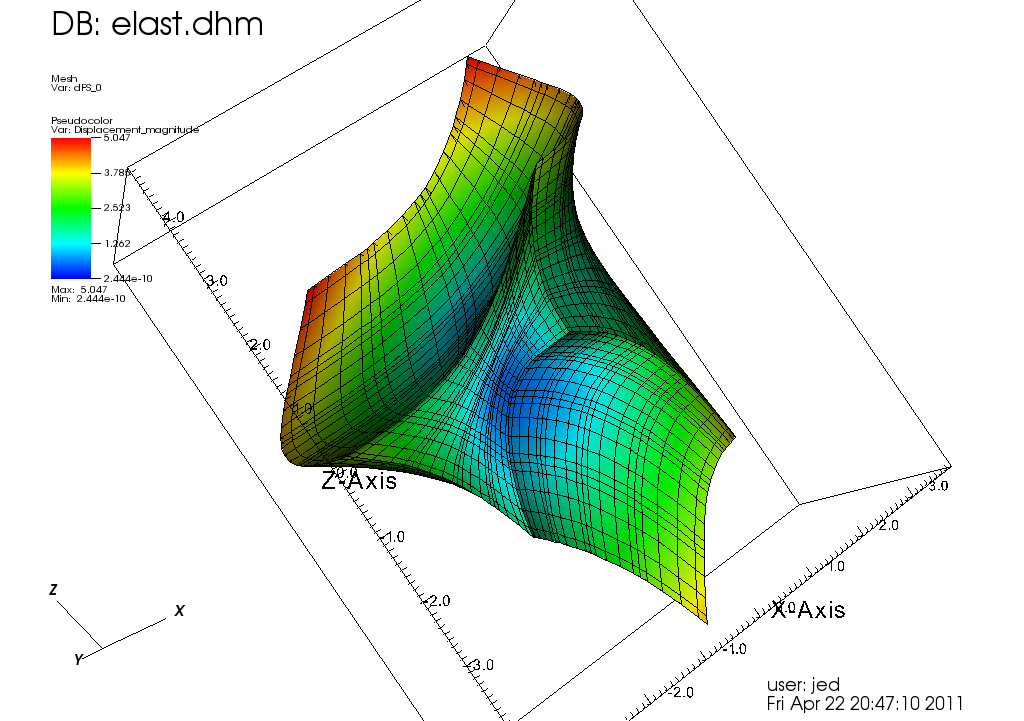
\includegraphics[width=\textwidth]{figures/elast-b4q5}
  \end{textblock}
  \begin{itemize}
  \item Manufactured solution
  \item Discretize with $Q_3$ elements
  \item Precondition with BoomerAMG
  \end{itemize}
\end{frame}

\begin{frame}{Numerical results: Elasticity}
  \begin{tabular}{llll llll}
  \toprule
  Method & Lag & LS & Linear Solve & Its. & $F(u)$ & Jacobian & $P^{-1}$ \\
  \midrule
  LBFGS & 3 & cp & \texttt{preonly} & 18 & 37 & 5 & 18 \\
  LBFGS & 3 & cp & \num{1e-05} & 21 & 43 & 6 & 173 \\
  LBFGS & 6 & cp & \texttt{preonly} & 24 & 49 & 4 & 24 \\
  LBFGS & 6 & cp & \num{1e-05} & 30 & 61 & 5 & 266 \\[1ex]
  \only<1>{
  Newton & 0 & bt & \texttt{preonly} & 13 & 14 & 13 & 13 \\
  Newton & 0 & bt & \num{1e-05} & 10 & 11 & 10 & 77 \\
  Newton & 0 & cp & \texttt{preonly} & 11 & 23 & 11 & 11 \\
  Newton & 0 & cp & \num{1e-05} & 8 & 17 & 8 & 60 \\
  Newton & 1 & bt & \texttt{preonly} & 16 & 21 & 8 & 16 \\
  Newton & 1 & bt & \num{1e-05} & 17 & 23 & 9 & 128 \\
  Newton & 1 & cp & \texttt{preonly} & 15 & 31 & 8 & 15 \\
  Newton & 1 & cp & \num{1e-05} & 13 & 27 & 7 & 103 \\
  Newton & 3 & cp & \texttt{preonly} & 23 & 47 & 6 & 23 \\
  Newton & 3 & cp & \num{1e-05} & 22 & 45 & 6 & 179 \\
  Newton & 6 & cp & \texttt{preonly} & 36 & 73 & 6 & 36 \\
  Newton & 6 & cp & \num{1e-05} & 35 & 71 & 5 & 294
}
\only<2>{
  JFNK & 0 & cp & \texttt{preonly} & 11 & 23 & 11 & 11 \\
  JFNK & 0 & cp & \num{1e-05} & 8 & 69 & 8 & 60 \\
  JFNK & 1 & cp & \texttt{preonly} & 15 & 31 & 8 & 15 \\
  JFNK & 1 & cp & \num{1e-05} & 7 & 2835 & 4 & 2827 \\
  JFNK & 3 & cp & \texttt{preonly} & 23 & 47 & 6 & 23 \\
  JFNK & 3 & cp & \num{1e-05} & 7 & 3143 & 2 & 3135
}
\end{tabular}
\end{frame}

\begin{frame}{Quasi-Newton}
  \begin{itemize}
  \item Quasi-Newton is effective for lagging setup
  \item Line search quality can make a big difference
  \item Still need good preconditioner to define $\tilde \vJ_0^{-1}$
  \item Usage in PETSc
    \begin{itemize}
    \item No code modification
    \item BFGS: \texttt{-snes\_type qn -snes\_qn\_restart\_type periodic -snes\_qn\_scale\_type jacobian}
    \item See \texttt{-snes\_qn\_type broyden} and \texttt{badbroyden}
    \item Support in PETSc 3.3, better in 3.4 (to be released Friday)
    \end{itemize}
  \item Non-symmetric problems
    \begin{itemize}
    \item BFGS needs symmetry, Broyden and Bad Broyden do not
    \item In testing, Broyden was rarely worse, but not a big win either
    \end{itemize}
  \item What goes wrong?
    \begin{itemize}
    \item Operator changes in a high-rank way (e.g., diagonal shift).
    \end{itemize}
  \item We plan to extend PETSc to support complementarity problems
  \end{itemize}
\end{frame}

\begin{frame}{Alternative: nonlinear solver composition}
  \begin{itemize}
  \item Nonlinear GMRES, Anderson mixing
    \begin{itemize}
    \item \texttt{-snes\_type ngmres}
    \end{itemize}
  \item Left nonlinear preconditioning
    \begin{equation*}
      \vu - \vG(\vF(\vu)) = 0
    \end{equation*}
  \item Right nonlinear preconditioning
    \begin{equation*}
      \vF(\vG(\vv)) = 0, \quad \vu = \vG(\vv)
    \end{equation*}
  \item Defining $\vG(\cdot)$ as a lagged linear solve moves ``Krylov'' acceleration to nonlinear problem
  \item General framework for nonlinear solver composition
    \begin{itemize}
    \item Accelerate and improve robustness of FAS multigrid
    \item Nonlinear domain decomposition (ASPIN is left-preconditioned Newton)
    \item \texttt{-snes\_type ngmres -snes\_npc\_side right -npc\_snes\_type fas}
    \end{itemize}
  \end{itemize}
\end{frame}

\begin{frame}{Beyond global linearization: FAS multigrid}
  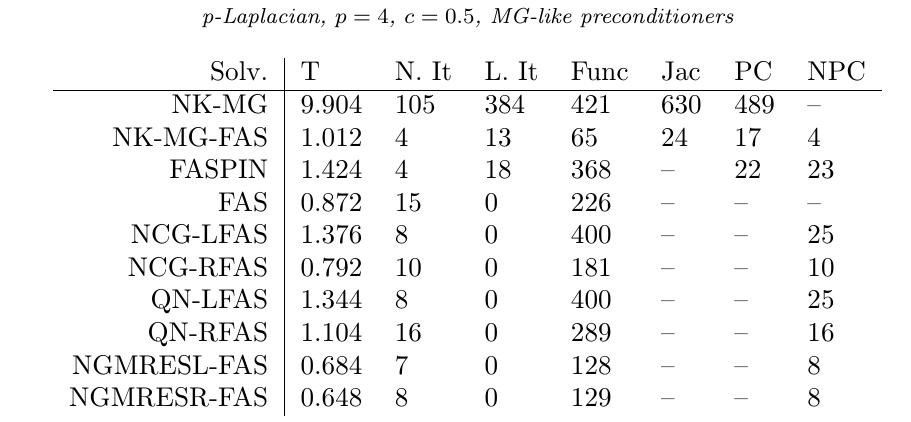
\includegraphics[width=\textwidth]{figures/BruneNGMRESFAS.png}
  \begin{itemize}
  \item Geometric coarse grids and rediscretization
  \end{itemize}
\end{frame}

\end{document}
